\section{\ourmethod: Data mixture as regression}

\begin{figure}[t]
    \vspace{-0.2cm}
    \centering
    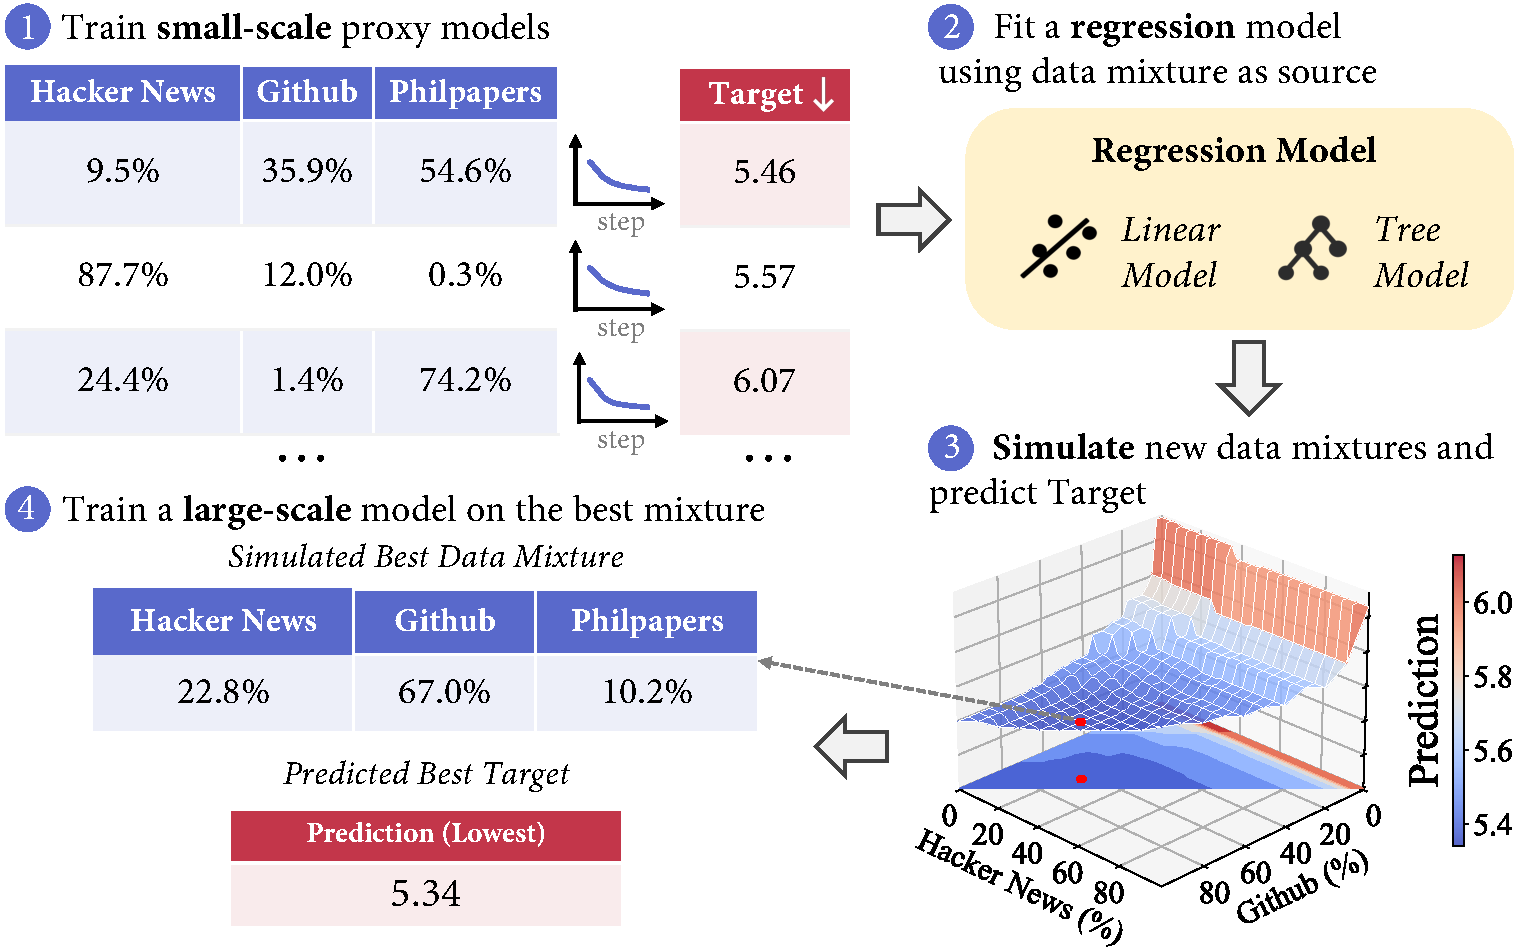
\includegraphics[width=0.9\textwidth]{figures/data_mixture_method_v9.pdf}
    \caption{The illustration of our method using Hacker News, GitHub, and Philpapers as training domains, with the loss on the StackExchange domain as the Target (where $\downarrow$ indicates lower is better). A regression model is fitted using small-scale proxy model training logs and employed to predict the best data mixture within the simulation space, enabling direct prediction of the data mixture for large-scale language model pre-training. Note that the Philpapers domain is omitted in the simulation plot (3) for simplicity.}
    \label{fig:method_overview}
    \vspace{-5mm}
\end{figure}

As illustrated in Figure~\ref{fig:method_overview}, our method involves four key steps: (1) Generate random data mixtures and train small-scale proxy models on these mixtures. (2) Fit a linear regression model using the mixtures as features and the target value as the label. (3) Simulate the data mixture space on a larger scale and leverage the regression model to identify the best mixture for the target value. (4) Train a large-scale model using the simulated best data mixture.

\subsection{Train small-scale proxy models}


The first step is to train a set of small-scale proxy models on multiple different data mixtures.
To reduce the required runs, we aim to select a diverse range of data mixtures that cover extreme weights from 0\% to 100\% for each domain.
We achieve this by using a Dirichlet distribution based on the token distribution, which allows us to sample a wide range of values and expose the regression models to various extremes.
Simultaneously, basing the distribution on the token distribution ensures that the overall data mixture statistically reflects the availability of data.
For example, this prevents any single domain with a token count below 1\% from being overly emphasized, which is not feasible for large-scale training since there are not enough available tokens from that domain.
In practice, we multiply the token distribution by a value from $0.1$ to $5.0$ to construct various sparse and near-uniform distributions, then use these distribution vectors as the Dirichlet distribution hyperparameter $\alpha$. \looseness=-1

After training small-scale proxy models for a few steps, we can obtain several well-trained small models. For example, in our main experiment, each proxy model contains 1M parameters and is trained on 1B tokens. We can then choose to evaluate these trained models on domains or benchmarks to get the target value we want to optimize.
Generally, the target value can be the loss on a domain, as shown in Figure~\ref{fig:method_overview} for the StackExchange domain.
Once we have obtained these target values, we can use the data mixture as features and the target values as labels to fit a regression model.

\subsection{Fit a regression model}

\begin{table*}[tb]
\centering
\small
\caption{Overview of the Pile dataset~\citep{the_pile_corpus} with datasets that are no longer available due to copyright issues marked in gray. In our experiments, we use the 17 available domains to study the data mixture for language model pre-training.}
\vspace{1mm}
\label{table:pile_overview}
\begin{tabular}{lr}
\toprule
\textbf{Component} & \textbf{Effective Size} \\
\midrule
Pile-CC  & 227.12 GiB  \\
PubMed Central & 180.55 GiB \\
\rowcolor{gray!25} Books3 & 151.44 GiB \\
\rowcolor{gray!25} OpenWebText2 & 125.54 GiB\\
ArXiv & 112.42 GiB \\
Github & 95.16 GiB\\
FreeLaw & 76.73 GiB \\
Stack Exchange & 64.39 GiB \\
USPTO Backgrounds & 45.81 GiB \\
PubMed Abstracts & 38.53 GiB \\
Gutenberg (PG-19) & 27.19 GiB \\
\bottomrule
\end{tabular}
\hspace{5mm}
\begin{tabular}{lr}
\toprule
\textbf{Component} & \textbf{Effective Size} \\
\midrule
\rowcolor{gray!25} OpenSubtitles & 19.47 GiB \\
Wikipedia (en) & 19.13 GiB \\
DM Mathematics  & 15.49 GiB \\
Ubuntu IRC & 11.03 GiB \\
\rowcolor{gray!25} BookCorpus2 & 9.45 GiB \\
EuroParl & 9.17 GiB \\
HackerNews & 7.80 GiB \\
\rowcolor{gray!25} YoutubeSubtitles & 7.47 GiB \\
PhilPapers & 4.76 GiB  \\
NIH ExPorter & 3.79 GiB  \\
Enron Emails & 1.76 GiB \\
\bottomrule
\end{tabular}
\vspace{-1mm}
\end{table*}

The second step is to fit a regression model using the data mixture as features, and the target value as labels.
The regression task is a conventional supervised learning task that involves predicting a continuous target variable $y$ based on input features $X = (x_1, x_2, \ldots, x_n)$. The goal is to find a function $f$ that best maps the input features to the target variable, such that $y=f(X) +\epsilon$, where $\epsilon$ represents the error or noise in the data. In the context of this paper, the input features $X$ correspond to the domain weights of the data mixture, and the target variable $y$ is the value we want to optimize. Using this data, we train regression models that learn a function to predict the target value based on arbitrary data mixtures without requiring further training.

\paragraph{Linear regression.}
The linear regression model is widely used in regression. It assumes a linear relationship between the input features and the target variable, which can be represented as:
\begin{equation}
y = \omega_0 + \omega_1 x_1 + \ldots + \omega_n x_n + \epsilon
\end{equation}
where $\omega_0$ is the intercept, and $\boldsymbol{\omega}=(\omega_1, \ldots, \omega_n)$ are the coefficients associated with the respective input features $x_1, \ldots, x_n$.
The coefficients $\boldsymbol{\omega}$ are typically estimated using techniques such as ordinary least squares, aiming to minimize the sum of squared residuals between the predicted and actual target values. In practice, we employ linear regression with L2 regularization, also known as ridge regression, which applies a penalty to the magnitude of $\boldsymbol{\omega}$ to prevent overfitting.

\paragraph{LightGBM regression.}
The LightGBM~\citep{ke2017lightgbm} is a powerful gradient-boosting algorithm that can be used for both regression and classification tasks. In the context of regression, LightGBM learns an ensemble of decision trees to predict the target variable. 
The process is guided by a gradient-based optimization algorithm, which minimizes a specified loss function (e.g. mean squared error). Moreover, LightGBM is designed to be efficient and scalable, making it suitable for large datasets.\looseness=-1

\subsection{Simulate and predict}

Once we have trained the regression model, we can efficiently explore the entire space of possible data mixtures.
By using the trained model to predict the target value for each potential data mixture, we can quickly identify the input that yields the best target value. This simulation-based optimization is relatively cheap, as both the simulation and the regression prediction are computationally fast. For example, running prediction for 1,000,000 data mixtures takes less than 10 CPU seconds.

\subsection{Large-scale model training}

After identifying the best data mixture with simulation, we generalize the top-ranked data mixture to a large-scale model training with many more tokens.  As shown in Figure~\ref{fig:method_overview}, we directly use the best data mixture for training the larger model. In practice, to increase the robustness of our regression prediction, we select the top $100$ mixtures and average them as the data mixture for large-scale training. \looseness=-1
